
% This LaTeX was auto-generated from MATLAB code.
% To make changes, update the MATLAB code and republish this document.

\documentclass{article}
\usepackage{graphicx}
\usepackage{color}

\sloppy
\definecolor{lightgray}{gray}{0.5}
\setlength{\parindent}{0pt}

\begin{document}

    
    
\section*{}


\subsection*{Contents}

\begin{itemize}
\setlength{\itemsep}{-1ex}
   \item PDF of 2 hypothesis; One without the target and other with the target
\end{itemize}


\subsection*{PDF of 2 hypothesis; One without the target and other with the target}

\begin{verbatim}
x = -10:0.001:10; % window for the normal distributon without the target
nu = 4;           % degrees of freedom for the chi squared distribution in the case of target present
x_c = 0:0.001:30; % window for chi squared distribution (because this distribution always starts from 0)

pd = makedist('Normal','mu',-1,'sigma',1); %Normal distribution object

pdf_norm = pdf(pd, x);                     %PDF of Normal distribution
pdf_chi = chi2pdf(x_c, nu);                %PDF of Chi Squared distribution


plot(x, pdf_norm, 'LineWidth', 2);         %Plot of Normal distribution
grid on;
hold on;

plot(x_c, pdf_chi, 'LineWidth', 2);        %Plot of Chi squared distribution

xlabel('x', 'FontSize', 12, 'FontWeight', 'bold');
ylabel('PDF', 'FontSize', 12, 'FontWeight', 'bold');
title('PDF of received signal', 'FontSize', 12, 'FontWeight', 'bold');
legend({'No target','With 1 target'},'Location','northeast', 'FontSize', 12, 'FontWeight', 'bold');
\end{verbatim}

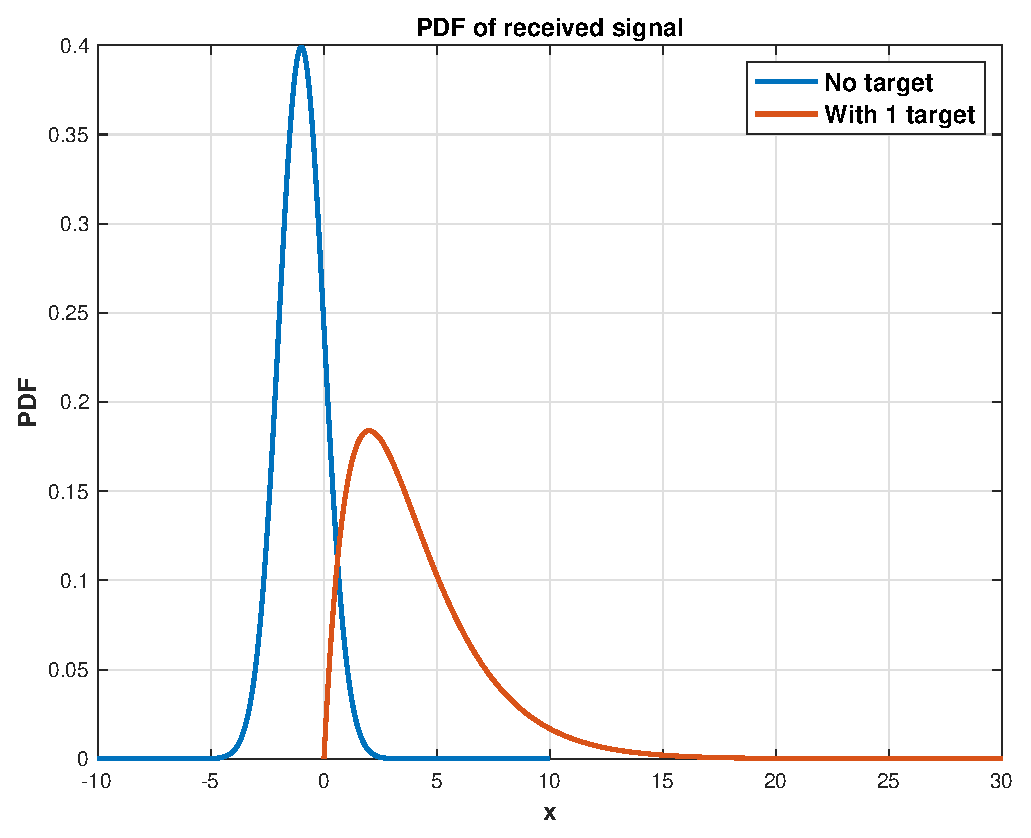
\includegraphics [width=4in]{pdf_m_01.eps}



\end{document}
    
